% Chapter 19: Charge and Electric Fields
\chapter{Charge and Electric Fields}

\step{A Counterintuitive Opening}

\begin{mainline}
On a winter night, you turn off the lights and remove a sweater in the dark. As it leaves your hair, tiny crackles sound and blue-white sparks flicker at the edge of your vision. Next morning, combing makes your hairs stand up and chase the comb. Touch a metal door handle and snap: a sharp shock strikes your fingertip.

Notice an overlooked oddity: there is no battery, outlet, or electrical appliance nearby. A sweater and plastic comb seem utterly unrelated to electricity. Yet they discharge it and even emit light.

Magnify this a millionfold: summer lightning illuminates half the stormy sky. What is lightning? By the end we can answer confidently. For now, it is the same physical process as your sweater's sparks on a different scale. Your bedroom stages miniature thunderstorms every night, unnoticed as a question.

This phenomenon has challenged people for over two millennia. Ancient Greeks found that amber rubbed with fur attracted feathers and straw. The Chinese character for electricity originally meant lightning. Yet only about two centuries ago did these scattered oddities become a coherent picture. We retrace that route from sweater sparks to the electric field: invisible and intangible, yet carrying force and energy. It is our first field in the full sense, the gateway to electromagnetism and ultimately to understanding light.
\end{mainline}

\step{Make a Guess First}

\begin{mainline}
Make three intuitive guesses without looking anything up, and write them down:

\begin{itemize}
  \item Rub a plastic ruler through your hair and bring it near paper scraps. They jump up. Once attracted, do they stay obediently attached?
  \item Rub two balloons through your hair, suspend them by threads, and bring them together. Do they attract, repel, or ignore each other?
  \item Rubbing charges objects. Is that electricity created by friction or transferred from somewhere? If created, where was it beforehand?
\end{itemize}

The third question sounds like wordplay but targets our deepest law. Almost everyone misses the first, assuming attracted means permanently attached. Reality is more interesting, hiding an entire microscopic relocation process.
\end{mainline}

\step{Hands-on Experiment}

\begin{experiment}[A Balloon's Static-Electricity Show]
You need an inflated balloon, fingernail-sized paper scraps, hair or a sweater, and a tap producing a very thin stream.

First, attract paper. Rub the balloon vigorously through hair about ten times, then hold it two or three centimeters above the scraps. They leap toward it. Watch for several seconds: some stick briefly, then abruptly jump off and fall. Remember this attract-then-repel sequence before seeking an explanation.

Second, stick it to a wall. Press the freshly rubbed balloon against the wall and release it. It stays for minutes on a flat, dry surface without glue or magnets. What force counters its weight?

Third, bend water. Adjust the tap to a thin continuous stream and bring the charged balloon nearby without touching. Water bends toward it as though pulled by an invisible hand. Water is neither paper nor iron; why is it attracted too?

Fourth, repelling balloons. Rub two balloons and suspend each by a thread. Bring them together and they visibly move apart. Why do identically treated balloons push each other away?

Safety: this experiment is entirely safe; any shock carries extremely little energy. But remember the corresponding contrast: static sparks are forbidden at filling stations, flour mills, and paint shops because of flammable vapors and dust. The same tiny spark has radically different consequences in different surroundings.
\end{experiment}

\step{The Old Model Runs into Trouble}

\begin{mainline}
So far, our pushes, pulls, pressures, springs, friction, and collisions have shared contact. Every force-diagram arrow seems to answer who touches the object. Gravitation acts at a distance, but cannot lift scraps for you; it is so weak that only giants such as Earth make it conspicuous. Apply this outlook to the balloon and trouble appears everywhere.

First, force crosses a gap. Paper jumps and water bends without balloon contact. Insisting on a touching agent requires inventing something invisible that pushes and pulls. That is exactly our task, but acknowledge that the old model has no place for it.

Second, the attracted objects apparently have no electricity. Paper, water, and wall were not rubbed and should be uncharged, yet are attracted. If only charged objects attract, why do they respond? Worse, two rubbed balloons repel. Neither attraction nor repulsion fits.

Third, electricity seems to come in two kinds. Historically, silk-rubbed glass and fur-rubbed rubber behaved differently. Two glass rods repelled, two rubber rods repelled, but glass and rubber attracted. The old model allows no two kinds: mass has one type and gravity only attracts.

Fourth, the books do not balance. Rubbing is never one-sided. As the balloon charges, your hair charges oppositely. Electricity appears in matching pairs, like debit and credit. If created, why exactly one pair every time?

Together these difficulties demand a new conserved, two-signed quantity; a new noncontact interaction, attractive or repulsive and astonishingly stronger than gravity; and a new carrier, the invisible thing that pushes.
\end{mainline}

\step{Inventing New Concepts}

\begin{mainline}
Invent them one at a time, as historical physicists did.

First: \textbf{electric charge}. Objects possess charge; like charges repel and unlike charges attract. Franklin named silk-rubbed glass's charge \textbf{positive} and fur-rubbed rubber's \textbf{negative}. These names are conventions; A and B would have worked, but once chosen, everyone must follow them.

Second: \textbf{charge conservation}. Rubbing transfers charge, not creates it. Negative particles move from hair to balloon, leaving the balloon negative and the hair equally positive. An isolated system's algebraic total remains constant: charge can relocate, not appear or vanish from nothing. This answers prediction 3 and the paired-charge puzzle: charging is separation. No exception has been found; it ranks with energy and momentum conservation among physics' firmest rules. Later, the carriers were identified as \textbf{electrons}, negatively charged atomic constituents easily removed or added. Positive protons normally remain tightly bound inside nuclei and do not make this move.

These are experimentally compelled ideas, not arbitrary inventions. Millikan's oil-drop experiment is especially revealing. Tiny charged droplets hang between metal plates; adjust the electric field to suspend one and use force balance to calculate its charge. Every result is an integer multiple of the same smallest amount, never half a step. Charge climbs discrete stairs whose unit is elementary charge \(e\), about \(1.6\times10^{-19}\) coulombs. Charge quantization is measured fact, not an assumption.

Third: \textbf{conductors and insulators}. Why does a metal handle shock you while a sweater does not actively do so? Materials treat charge differently. Metals have many freely roaming electrons, letting charge spread and flow immediately: \textbf{conductors}. Rubber, plastic, and dry hair lock charge in place: \textbf{insulators}. Conductors resemble paved roads, insulators separate drawers. Hence copper wire inside plastic: one carries electricity, the other confines it. Your conducting hand touching a winter door handle lets accumulated sweater charge discharge suddenly, producing the snap.

Fourth, solving uncharged attraction: \textbf{polarization}. Paper initially mixes positive and negative charge evenly with zero total. A nearby charged balloon repels or attracts negative charges, shifting them slightly at atomic scales. The paper remains neutral but becomes a tiny needle with slightly positive and negative ends. Its nearer end has opposite sign and stronger attraction; the farther, same-sign end has weaker repulsion. Distance dependence favors attraction overall. Bending water and wall-sticking balloons share this mechanism: \textbf{a charged object needs not a charged partner, only a slight rearrangement of the partner's charges}. Attraction of light neutral objects is a consequence of induced polarization, not an exception.

These concepts solve another historical puzzle: why electricity follows rubbing. The key is contact and separation, not rubbing itself. Different materials in close contact have different affinities for electrons; separation leaves some on the more acquisitive side. Rubbing enlarges contact area and repeats contact, accumulating transfers. Dry winter air makes it conspicuous because moisture otherwise leaves a thin conductive surface film that quietly drains charge. Static is therefore a specialty of dry weather.

Charge conservation also has precise experimental support. In Faraday's ice-pail experiment, a charged ball on silk thread is lowered into a metal bucket connected to an electrometer without touching its walls. The meter deflects as the ball enters, remains unchanged as it moves inside, and returns to zero when removed. Charge induced outside exactly matches the enclosed ball's charge. It neither multiplies during induction nor is swallowed by the bucket; it rearranges between inner and outer surfaces. Later tests reached extraordinary precision, and conservation remains unbroken.
\end{mainline}

\step{The Model in One Sentence}

\begin{oneline}
Charge is a conserved positive-or-negative property, with like signs repelling and unlike signs attracting; it acts through a space-filling electric field, first changing the surrounding spatial state, which then pushes or pulls other charges without contact.
\end{oneline}

\step{The Mathematical Translator}

\begin{mainline}
With concepts assembled, translate them into calculable expressions.

First, force magnitude. Coulomb made precise torsion-balance measurements, suspending a charged ball from an extremely thin quartz fiber and bringing another nearby. Electrical force twists the fiber through an angle proportional to force, a turning balance weighing forces smaller than a speck of dust. The result: force between point charges is proportional to their charge product, inversely proportional to separation squared, and directed along their joining line. Like signs repel; unlike attract:

\[ F = k\,\frac{|q_1 q_2|}{r^2},\qquad k \approx 9.0\times 10^{9}\ \mathrm{N\cdot m^2/C^2} \]

The formula gives the force between charges. The product \(q_1 q_2\) records how much each carries; doubling either doubles force. The denominator \(r^2\) makes force shrink with distance squared. The SI charge unit is the coulomb, C.

Immediately check special cases:

\begin{itemize}
  \item Infinite separation makes \(F\) tend to zero: sufficiently distant charges barely interact.
  \item Zero charge on either side gives zero direct Coulomb force. Paper polarization creates local charges rather than violating this statement.
  \item Halving distance quadruples force, the inverse-square behavior precisely tested by the balance.
  \item Reverse positions: force magnitude stays the same while direction reverses, matching Newton's third-law action and reaction.
  \item Zero separation gives infinite force. This is an alarm, not a prediction: real charges are not mathematical points, and the formula fails at close range. Our limits section addresses it.
\end{itemize}

Compare gravity. Both are inverse-square, noncontact long-range forces. But mass has one kind, gravity always attracts and cannot be shielded, while charge has two signs, neutralizes, and can be shielded. Their strengths differ absurdly: proton--proton electric repulsion is about \(10^{36}\) times gravitational attraction. Gravity rules the cosmos only because large-scale positive and negative charge nearly cancel, while gravity does not.

Second comes our central concept, the \textbf{electric field}. Coulomb tells us two charges push each other, not how that push crosses space. Faraday transformed physics by asking not how A pushes B, but what A does to surrounding space. At every point define a vector, electric field strength, equal to force per coulomb on a positive charge there, directed as that force:

\[ \mathbf E = \frac{\mathbf F}{q_{\text{test}}} \]

Its unit is newtons per coulomb, N/C. The imagined \(q_{\text{test}}\) is a \textbf{test charge}, small enough to negligibly disturb the original field, like a float measuring flow without changing it. Force calculation now has two stages: the source creates \(E = kQ/r^2\), outward or inward around a point charge, then the field exerts \(\mathbf F = q\mathbf E\). A negative charge feels force opposite the field.

Third is \textbf{superposition}: the field of several charges is the vector sum of their separate fields. Almost trivial sounding, it is enormously powerful. Divide any complicated charged body into little pieces, calculate each field, and add. Nearly every calculation here and in Chapter 20 rests on this sentence.

We depict invisible fields with \textbf{field lines}, curves tangent everywhere to the local field direction, drawn more densely where it is stronger. A point charge's lines radiate outward or converge inward, spreading with distance. Spherical area grows as \(r^2\), so line density falls as \(1/r^2\), matching Coulomb exactly. This is no coincidence and hints at a deeper statement shortly.
\end{mainline}

\begin{figure}[htbp]
\centering
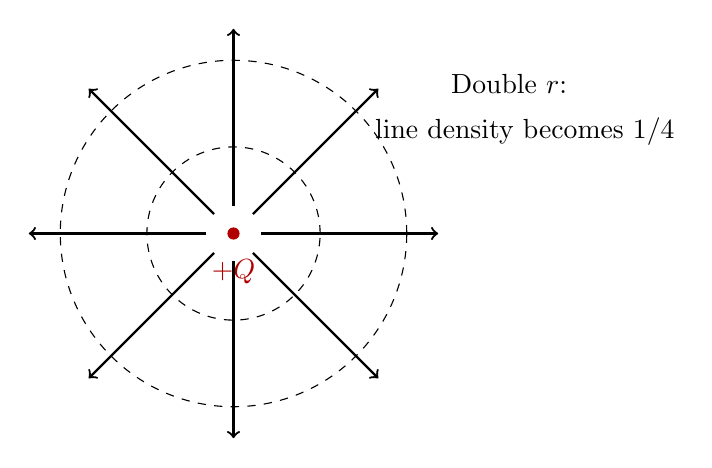
\begin{tikzpicture}[scale=1]
  \fill[red!70!black] (0,0) circle (2.2pt) node[below=6pt] {$+Q$};
  \foreach \a in {0,45,...,315}
    \draw[->,thick] ({0.35*cos(\a)},{0.35*sin(\a)}) -- ({2.6*cos(\a)},{2.6*sin(\a)});
  \draw[dashed] (0,0) circle (1.1);
  \draw[dashed] (0,0) circle (2.2);
  \node at (3.5,1.9) {Double $r$:};
  \node at (3.7,1.3) {line density becomes $1/4$};
\end{tikzpicture}
\caption{A positive point charge's field lines radiate outward, becoming sparser with distance in proportion to \(1/r^2\).}
\end{figure}

\begin{mainline}
An estimate reveals how enormous a coulomb is. Two small balls each carry one coulomb, one meter apart:

\[ F = 9.0\times10^{9}\ \mathrm{N} \]

Nine billion newtons, the weight of about 900,000 tonnes, roughly two skyscrapers pressing across a meter. Conversely, rubbing a balloon transfers only around \(10^{-8}\) coulombs, about \(10^{11}\) electrons, against roughly \(10^{23}\) surface atoms. Moving just one electron per trillion suffices to support it on a wall and bend water remotely. Together these estimates explain everyday neutrality: the electrical force coefficient is so large that slight macroscopic net charge would create overwhelming forces, so nature strongly balances the signs. Rare, striking static effects are tiny occasional failures of that balancing process.

Finally, the intuitive version of beautiful \textbf{Gauss's law}, too easily skipped as advanced mathematics. Imagine a fluidlike field with charges as sources or sinks: positive springs pour out lines, negative drains collect them. Surround a source with any closed surface, spherical, box-shaped, or potato-like. \textbf{The total net field-line outflow depends only on enclosed net charge, not the surface's shape, size, or position}. More enclosed positive charge means more net outflow; balanced signs mean zero. Counting enclosed charge through outward flux is Gauss's idea. It resembles counting a room's occupants by entry-minus-exit records instead of tracking positions. It differs from real fluid counting: a field is not material flow, and flux measures its passage through an abstract surface without anything actually flowing.
\end{mainline}

\begin{mathbridge}
Write this intuition and see its efficiency under symmetry. Define closed-surface \textbf{electric flux} as \(\varPhi_E=\oint \mathbf E\cdot d\mathbf A\), summing each small area vector dotted with the field, outward positive and inward negative. Gauss's law says

\[ \varPhi_E=\oint \mathbf E\cdot d\mathbf A=\frac{Q_{\text{inside}}}{\varepsilon_0},\qquad \varepsilon_0\approx 8.85\times10^{-12}\ \mathrm{C^2/(N\cdot m^2)} \]

For spherical symmetry, surround point charge \(Q\) with a sphere of radius \(r\). The field \(E\) has equal magnitude everywhere and is radial, giving \(\varPhi_E = E\cdot 4\pi r^2 = Q/\varepsilon_0\). Thus

\[ E=\frac{Q}{4\pi\varepsilon_0 r^2} \]

Coulomb's inverse square follows from conserved flux and spherical area growing as \(r^2\). Our three-dimensional world is written into \(1/r^2\).

For an infinite uniformly charged plane, symmetry makes the field perpendicular everywhere and independent of distance. A cylinder crossing the plane receives \(EA\) flux through each end and none through its sides. Hence \(2EA=\sigma A/\varepsilon_0\), giving

\[ E=\frac{\sigma}{2\varepsilon_0} \]

Independent of distance: an infinite plane produces a uniform field. Doubling distance does not halve it, a counterexample to unqualified inverse-square intuition. Chapter 20's capacitors use two such planes to create uniform fields.
\end{mathbridge}

\begin{figure}[htbp]
\centering
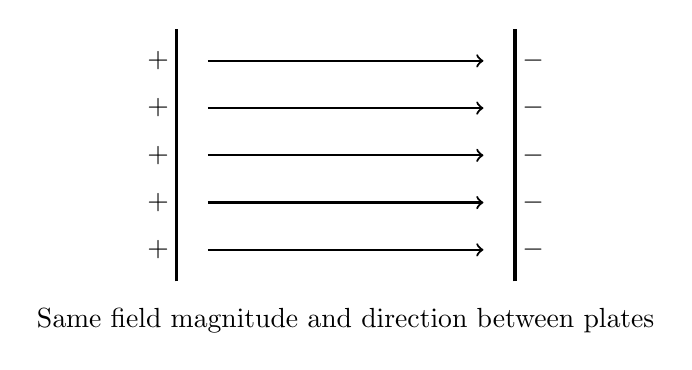
\begin{tikzpicture}[scale=1]
  \draw[very thick] (-0.15,-1.6) -- (-0.15,1.6);
  \draw[very thick] (4.15,-1.6) -- (4.15,1.6);
  \foreach \y in {-1.2,-0.6,0,0.6,1.2}
    \node at (-0.38,\y) {$+$};
  \foreach \y in {-1.2,-0.6,0,0.6,1.2}
    \node at (4.38,\y) {$-$};
  \foreach \y in {-1.2,-0.6,0,0.6,1.2}
    \draw[->,thick] (0.25,\y) -- (3.75,\y);
  \node at (2,-2.1) {Same field magnitude and direction between plates};
\end{tikzpicture}
\caption{Oppositely charged parallel plates have parallel, equally spaced field lines between them: a uniform field.}
\end{figure}

\begin{mathbridge}

Conductor equilibrium follows in one sentence. An internal field would move free electrons until their rearrangement cancels it. Thus electrostatic equilibrium has \(E=0\) inside the conductor and all charge on its surface. This underlies metal enclosures' electrostatic shielding.
\end{mathbridge}

\begin{challenge}
Gauss's integral law also has a local differential form, \(\nabla\cdot\mathbf E=\rho/\varepsilon_0\): field divergence at a point equals charge density divided by \(\varepsilon_0\). It identifies sources point by point without an imagined closed surface.

A thread for later: Coulomb describes a present source position and a force elsewhere as though transmission took no time. If A suddenly moves, does B know immediately? That would violate the deeper limit that no influence exceeds light speed, discussed in relativity. Treating the field as physically real resolves this. A's disturbance propagates through the field at light speed; B responds only on its arrival. Once fields carry messages, Chapter 22's magnetism, Chapter 24's Maxwell equations, and Chapter 25's electromagnetic light follow in sequence. Is the field real? It carries energy and momentum and can be emitted to travel independently, satisfying physics' strictest practical criteria for reality.
\end{challenge}

\step{The Model's Limits}

\begin{mainline}
As usual, state where each model applies or fails, and distinguish experimental fact, mathematical model, and physical explanation.

Coulomb's limits: it describes \textbf{stationary} point charges or spherically symmetric distributions, repeatedly tested with high precision from atomic to macroscopic scales. Three departures matter. Moving charges introduce velocity-dependent magnetic force, Chapter 22's subject; Coulomb covers only the static part. Vanishing separation produces divergence, exposing point-charge idealization: real distributions require piecewise superposition at close range. And charge is quantized: free charge comes in integer multiples of \(e\approx1.6\times10^{-19}\) C. Treating \(q\) continuously is fine macroscopically because \(e\) is tiny, but half an electron's charge is not a valid question about an individual electron.

Field-line limits: these are drawings, not objects. No literal bundles of threads fill space. Density representing strength is a drawing convention, strictly corresponding to flux only under particular constructions. Lines never cross, or one point would have two field directions. They begin on positive charges and end on negative ones or extend to infinity. Electrostatic lines never close, a condition Chapter 23's changing-magnetic-field-induced electric fields will break. Treating lines as literal vibrating, stretched strings overinterprets them.

Limits of the field explanation: experiments measure forces as Coulomb describes; mathematical models are Coulomb, superposition, and Gauss; the physical explanation is a spatial field transmitting interaction. Do not conflate them. In accessible static experiments, action at a distance calculates the same forces, a historical view some defended. We call fields real because motion and change expose that view's failures: varying fields carry energy and propagate at finite speed, verified experimentally. This is a classic explanation promoted to fact by new evidence, illustrating why we distinguish the levels.

Two common misuses: a test charge is no new kind of charge, only a measuring tool, like a thermometer that should not heat the soup. And Gauss's law does not require symmetry to hold. It is exact for every distribution and closed surface. Without symmetry it simply seldom determines \(E\) by itself, requiring superposition or fuller equations.
\end{mainline}

\step{Explaining the Opening Phenomenon}

\begin{mainline}
Return to the winter bedroom and unpack the spark's sequence.

Act 1, separation: sweater and hair repeatedly contact and rub throughout the day, transferring electrons between materials. Net charge accumulates; even around \(10^{-8}\) coulombs creates a substantial field. Dry winter conditions provide no watery surface escape route, so charge keeps building.

Act 2, field growth: removing the sweater suddenly separates charged layers. Charges are already separated and distance grows, strengthening the field between signs. Across narrow hair--sweater gaps, field strength can exceed hundreds of thousands of volts per meter.

Act 3, breakdown: air normally insulates, but only up to a limit. At about \(3\times10^{6}\) N/C, equivalently three million volts per meter, rare free electrons accelerate and knock out more electrons in an avalanche. Air abruptly conducts: breakdown. Charge discharges through the new channel, releasing light and sound, the blue-white spark and crackle.

Act 4, scaling up: lightning uses the same script with clouds. Convecting, colliding ice crystals and droplets separate and accumulate charge. Cloud--ground fields strengthen until kilometers of air break down. One flash can transfer tens of coulombs and release billions of joules. Bedroom sparks and thunderbolts differ in scale, not physics.

The remaining phenomena also fit. A balloon polarizes a wall, inducing opposite charge nearby that holds it. Paper is first polarized and attracted, then receives same-sign charge on contact and is repelled; those predicting permanent attachment can now grade themselves. A door-handle snap is a miniature breakdown discharging your body's accumulated charge through your finger into metal. Water molecules already have slightly positive and negative ends; they turn collectively in the field and are pulled toward the balloon.

Other everyday static puzzles follow. Old CRT television and computer screens collect dust because their charge attracts airborne particles. Synthetic skirts cling to legs in autumn and winter because repeated contact separates charges that attract. Printers sometimes take several sheets together because dry sheets accumulate same-sign charges and stick. Barbershop hair scraps follow combs for the same reason as the opening sweater. Recognize charge separation, polarization, and discharge, and winter becomes your laboratory.

Technology grows from the same tree. Electrostatic precipitators charge smokestack dust in strong fields, then collect it on oppositely charged plates. Copiers and laser printers use light to write electrostatic patterns on photosensitive drums, attracting toner for transfer to paper. Every photocopy was once drawn with a field. Reverse engineering matters too: grounding chains on fuel tankers, touching a discharge point before refueling, and discharging aircraft before landing all assist charge balancing and prevent sparks in dangerous places.
\end{mainline}

\step{Thought Experiments and Challenges}

\begin{thought}[What If Proton and Electron Charges Differed Slightly?]
Experiments find proton and electron charge magnitudes equal to better than \(10^{-21}\), with no measured difference. Suppose electron charge were smaller by one part in a billion, \(10^{-9}\). What would happen?

Your body contains around \(10^{28}\) protons. An average surplus of \(10^{-9}\) elementary positive charges per proton would give net charge about \(1.6\) coulombs. Recall that two one-coulomb charges a meter apart repel with nine billion newtons. You and another person would each carry coulomb-scale charge and repel with landslide-like force. Forget handshakes: you could not share a room. Earth would also charge; celestial repulsion would overwhelm gravity, rewriting galaxies, planets, and atomic chemical bonds.

This is not merely a close-call story. Our world's existence depends on extraordinarily precise charge balance. Why are electron and proton magnitudes exactly equal? Physics has not completely answered; grand unified theories grew partly from such questions.
\end{thought}

\begin{puzzles}
  \item A balloon attracts paper that jumps off seconds later. Someone says its electricity ran out. Why is that wrong? Retell the process using charge conservation and contact charging.\\
  \textbf{Hint:} charge relocates rather than running out. Follow electrons from balloon to paper: what charge did the paper have before contact, and afterward?
  \item Fix two identical charged balloons symmetrically on a table and suspend a third charged ball midway between them, where net force is zero. Nudge it sideways and release. Does it return or move farther away? How does this zero-force location differ from a ball at a bowl's bottom?\\
  \textbf{Hint:} draw both Coulomb forces after displacement; the nearer charge's force increases by the inverse-square rule. Compare restoration with further displacement. This hints at the general theorem that electrostatic forces alone provide no stable equilibrium point.
  \item Enclose a playing radio in metal mesh and its sound weakens or disappears; plastic mesh has little effect. Explain using conductor electrostatic equilibrium, and why mesh holes need not form solid sheet metal to work reasonably well.\\
  \textbf{Hint:} free charges rearrange to cancel the internal field. Shielding requires holes much smaller than the changing field's spatial scale, a clue made precise in Chapter 25.
  \item Gauss's intuition says net flux through a closed surface depends only on enclosed charge. Would this remain true if Coulomb force fell as \(1/r^3\) instead? Compare two concentric spheres around a point charge.\\
  \textbf{Hint:} flux is field strength times spherical area. If \(E\) falls as \(1/r^3\), what are the inner and outer fluxes, and do they match? Inverse square is not a coincidence but a prerequisite for conserved flux, or the signature of three-dimensional space.
\end{puzzles}
